\documentclass[crop,tikz]{standalone}% 'crop' is the default for v1.0, before it was 'preview'
% %\usetikzlibrary{...}% tikz package already loaded by 'tikz' option
\usetikzlibrary{calc,patterns,angles,quotes}
\begin{document}
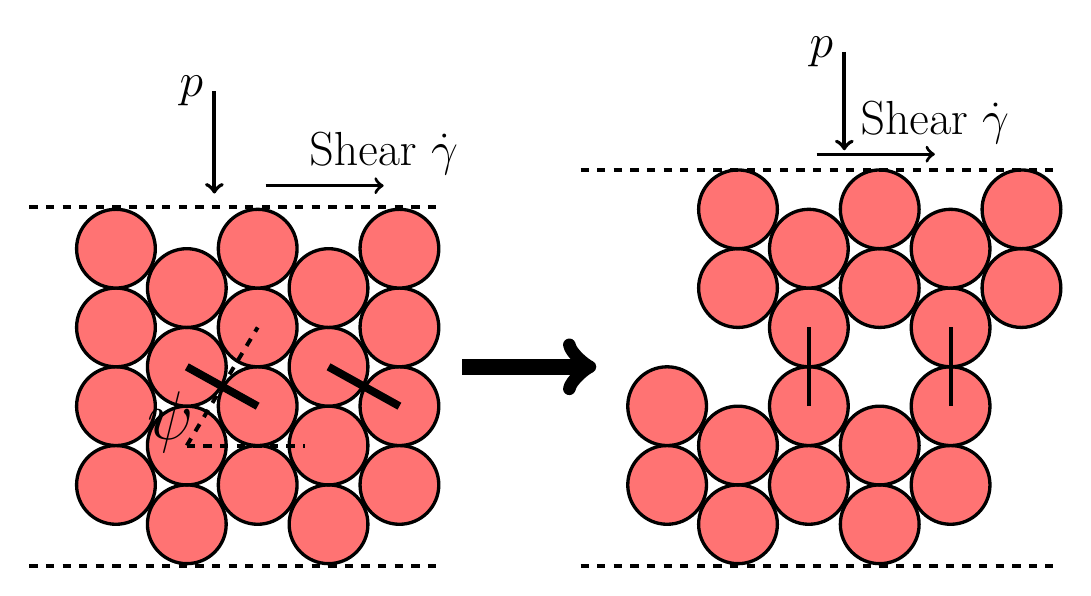
\begin{tikzpicture}[scale = 1.]
    % \draw (-11.5,4) node {\textbf{A}};
    % \draw (-1.5,4) node {\textbf{B}};

    \def \b {7};
    \def \c {-7};
    \def \d {0.1};
    \def \r {0.5};

    % Before dilatancy
    \foreach \x in {1.1, 2.9, 4.7}
        \foreach \y in {1.5,..., 4.5}
            \draw [color=black, fill=red!55,very thick] (\x, \y) circle (0.5);

    \foreach \x in {2, 3.8}
        \foreach \y in {1,..., 4}
            \draw [color=black, fill=red!55,very thick] (\x, \y) circle (0.5);

    %contact forces
    \draw[ very thick, line width = 1mm] (2.9, 2.5) -- (2,3);
    \draw[ very thick,line width = 1mm] (4.7, 2.5) -- (3.8,3);
    
    \draw[dashed, very thick] (0, 5.03) -- (5.2,5.03);
    \draw[dashed, very thick] (0, 0.47) -- (5.2,0.47);

    % \draw[->, very thick, line width = 1mm]  (0.1, 4.2) node[left] {\LARGE $p$} -- (0.1, 5.03) ;
     
    \draw [very thick, ->] (3, 5.3) -- (4.5, 5.3) node[above] {\LARGE Shear $\dot\gamma$};

        \draw[->, very thick, line width = 0.5mm]  (2.35, 6.5) node[left] {\LARGE $p$} -- (2.35, 5.2) ;

    \draw[->, line width = 2mm] (5.5, 3) -- (7.2,3);
    
    %When dilatating
    
    \foreach \x in {1.1, 2.9, 4.7}
        \foreach \y in {1.5,2.5}
            \draw [color=black, fill=red!55,very thick] (\x+\b, \y) circle (0.5);

    \foreach \x in {2, 3.8}
        \foreach \y in {1,2}
            \draw [color=black, fill=red!55,very thick] (\x+\b, \y) circle (0.5);

    \foreach \x in {2.9, 4.7}
        \foreach \y in {3.5, 4.5}
            \draw [color=black, fill=red!55,very thick] (\x+\b, \y) circle (0.5);

    \foreach \x in {2, 3.8, 5.6}
        \foreach \y in { 4,5}
            \draw [color=black, fill=red!55,very thick] (\x+\b, \y) circle (0.5);

    \draw[dashed, very thick] (0+\b, 0.47) -- (6+\b,0.47);
    \draw[dashed, very thick] (0+\b, 5.5) -- (6+\b,5.5);


    \draw[->, very thick, line width = 0.5mm]  (3.35+\b, 7) node[left] {\LARGE $p$} -- (3.35+\b, 5.75) ;
     
    \draw [very thick, ->] (3+\b, 5.7) -- (4.5+\b, 5.7) node[above] {\LARGE Shear $\dot{\gamma}$};

    \draw[ very thick, line width = 0.5mm] (2.9+\b, 2.5) -- (2.9+\b,3.5);
    \draw[ very thick,line width = 0.5mm] (4.7+\b, 2.5) -- (4.7+\b,3.5);

    \coordinate (A) at (4, 2);
    \coordinate (B) at (2, 2);
    \coordinate (C) at (2.2, 2.4);
    \draw[dashed, thick, line width = 0.5mm] (2, 2) -- (3.5, 2);
    \draw[dashed, thick, line width = 0.5mm] (2, 2) -- (2.9, 3.5);
    \pic [draw, -,, angle eccentricity=1.5] {angle = A--B--C};
    
    \node[color = black] at (1.8, 2.3)  {\Huge $\psi $};
    % \node at (0, 6)  {\LARGE (a) $\psi > 0$};

\end{tikzpicture}

\end{document}